% ============================================================
% S2 导学件量产·试点首件 —— 1.1.1 第2课时 空间向量的数量积（课时2 导学件）
% 轮4 成卷·S2｜2026-09-12｜生成链：xelatex main.tex（两遍）→ python render.py（150dpi → png/pageN.png）
%
% 模板承 v11 样张族 `工作区/字替对照-0909/靠齐样张-0910/导学增量/`：
%   qp-fonts/qp-layout/qp-parts/qp-headfoot/qp-titles/qp-blocks 六宏＝原样拷贝（L1 冻结参数零改动）；
%   课时页形制（\keshi→【学习目标】→双栏：课前预习(知识导学填空＋诊断分析挂每个知识点后)
%   →课中探究(探究点·题型名：例1→变式1→素养小结)→课堂评价恒5（\vbox 整体装栏）＋书写留白水印）
%   与局部宏（\pingtou/\liubai/\zhankong）照抄 导学增量/main.tex；chapterhead.tex 随件拷贝备档，本件未用。
% 图＝源图位图（禁绘三维，公共规则§5；figs/ 三件取自样张族 variantF/media/media/ 原图，未改绘）。
%
% 取材链登记（S2 试点侦察结论，详见 成卷/导学件/S2就绪报告.md）：
%   ① 课中探究 例1/变式1/素养小结＝v11 冻结导学件（variantF/body.tex 探究点五~九）**逐字同文**，
%      件内重编为探究点一~五（全品式号段「例N/变式N 探究点内」不受影响）；
%      对应关系：一←v11五(数量积概念与运算律) 二←v11六(求夹角与投影) 三←v11七(条件求参)
%                四←v11八(求距离·展开法) 五←v11九(求距离·折叠矩形)。
%   ② 课前预习 ZSD一/三 条目＝v11 同文（body.tex 知识点三 夹角/投影条目，含编注）；
%      ZSD二 tiaomu2「数量积运算律」＝教材 1.1.1 数量积性质(4)(5)(6) 逐字化用（白名单·教材原文挖空）；
%      ZSD二 判断(1)＝v11 同文；其余判断题 5 条＋课堂评价 5 题＝本轮命制（白名单口径，逐题亲算
%      登 成卷/导学件/S2就绪报告.md 附录；3 单选＋2 填空、难度≤例题、填空带提示词＝G5 内构）。
%   ③ 与练习轴课时02 十六题（题面库/课时02-1.1.1课2.md）零同文重合：讲部 1.1.1 十题例题位
%      已全部随 v11 冻结，课时2 域讲部新增可用＝0；重合复核（A-2/A-4 跨件口径）见就绪报告 §二。
%   ④ 顺手勘误（非 L1 参数，仅正文文句）：v11 知识点三·数量积条目编注重复读「零向量与任意向量的
%      数量积为0」两遍，本件并入一条；差异留痕见就绪报告 §三。
% 编译门：三 0（error＝0／Overfull＝0／Missing character＝0）——复跑命令与结果见就绪报告 §四。
% ============================================================
\documentclass[fontset=none]{ctexart}
\usepackage{qp-m3} % 换装：六宏→qp-m3 单包（钉后版 md5 7c3930362be8a0a2bdf21bbf8ac16573，两补钉随版）

% ================= 页脚参数宏（qp-headfoot 文件头明示的复用入口，非模块语义改动） =================
\renewcommand{\qpzhangming}{第一章\quad 空间向量与立体几何}
\renewcommand{\qpjianming}{导学件}
\renewcommand{\qpceming}{高中数学\quad 选择性必修第一册(人教B版)} % 换装回钉：qp-m3 默认册名＝选必二，防页脚漂移（试迁规约）

% ================= 局部宏（照抄 v11 导学增量/main.tex 冻结定义；不动公共模块） =================
% 课堂评价组头（XB-02 \zhenhead 同构：\biaoqian 1.3× 标签＋仿宋说明行；恒 5 题说明）
% 局部宏 \pingtou 已由 qp-m3 收编（等值定义），依换装方案§1.4 预删防撞名
% 书写留白＋斜置浅灰水印（导学案正文属性：答案另册→正文留书写位；斜置 25°／black!12）
% 长度 \liubaoh 已由 qp-m3 分配，预删防重复定义
% 局部宏 \liubai 已由 qp-m3 收编（等值定义），依换装方案§1.4 预删防撞名
% 纯书写占位留白（无水印）
% 局部宏 \zhankong 已由 qp-m3 收编（等值定义），依换装方案§1.4 预删防撞名

% 纯题版孤行抑制（正装三裁①）：小结②操作/③收束独立段，pure 档整段隐藏，含详解版不受影响
\newcommand{\bindpx}[1]{\ifshowans\bindp{#1}\fi}

\begin{document}
%成书重装五本跨本连续页码（G7方案B，承M2/M3装配先例）setcounter 注入位
\setcounter{page}{8}

% ============================================================
% 课时页（第2课时；五段闭环，承 v11 导学增量课时页样板形制）
% ============================================================
\keshi{第2课时\quad 空间向量的数量积}
\mubiaoline
\mubiaomu{1}{理解空间向量夹角、数量积与投影向量的概念，掌握数量积的运算律；}
\mubiaomu{2}{会用数量积(基底法)求空间向量的夹角与投影向量；}
\mubiaomu{3}{掌握用数量积求空间中两点间的距离(展开法与折叠模型)，体会向量运算的几何本质.}

\vspace{1.7mm}
\begin{multicols}{2}
\emergencystretch=1em

% ---------- 课前预习（知识导学填空＋诊断分析挂每个知识点之后） ----------
\huaxing{课}{前}{预}{习}{知识导学\quad 素养初识}

\zsd{一}{空间向量的夹角}

\tiaomu{1}{夹角：已知两个非零向量\(\overrightarrow{a},\overrightarrow{b}\)，在空间中任取一点\(O\)，作\(\overrightarrow{OA}=\overrightarrow{a},\overrightarrow{OB}=\overrightarrow{b}\)，则大小在\kongbai{}内的\(\angle AOB\)称为\(\overrightarrow{a}\)与\(\overrightarrow{b}\)的夹角，记作\(\langle\overrightarrow{a},\overrightarrow{b}\rangle\)；当\(\langle\overrightarrow{a},\overrightarrow{b}\rangle=\frac{\pi}{2}\)时，称\(\overrightarrow{a}\)与\(\overrightarrow{b}\)\kongbai{}，记作\(\overrightarrow{a}\perp\overrightarrow{b}\).\zhuzhu{夹角范围(0°到180°)是数量积正负讨论的前提；易混点：几何角(如异面直线所成角)与向量夹角可能互补，运算前先分清求的是哪个角.}}

\zhenhead{判断正误(正确的打\gou{},错误的打\cha{})}

\zhentib{(1)}{两个非零空间向量的夹角大小与这两个向量起点的位置有关．}

\begin{ansblock}[导-课时02-判1]
% ans:导-课时02-判1
\ansitem{(1)}{$\times$}
\end{ansblock}

\zhentib{(2)}{空间向量的夹角与异面直线所成角的取值范围相同．}

\begin{ansblock}[导-课时02-判2]
% ans:导-课时02-判2
\ansitem{(2)}{$\times$}
\end{ansblock}

\zsd{二}{空间向量的数量积}

\tiaomu{1}{数量积：定义\(\overrightarrow{a}\cdot\overrightarrow{b}=|\overrightarrow{a}||\overrightarrow{b}|\cos\langle\overrightarrow{a},\overrightarrow{b}\rangle\)；规定\kongbai{}与任意向量的数量积为0．性质：\(\overrightarrow{a}\perp\overrightarrow{b}\Leftrightarrow\overrightarrow{a}\cdot\overrightarrow{b}=0\)；\(\overrightarrow{a}\cdot\overrightarrow{a}={{\overrightarrow{a}}^{2}}={| \overrightarrow{a} |}^{2}\)；\(| \overrightarrow{a}\cdot\overrightarrow{b} |\leq| \overrightarrow{a} || \overrightarrow{b} |\).\zhuzhu{求空间角与距离的核心运算；注意数量积不满足结合律，零向量与任意向量的数量积为0.}}

\tiaomu{2}{运算律：\(\overrightarrow{a}\cdot\overrightarrow{b}=\)\kongbai{}(交换律)；\((\lambda\overrightarrow{a})\cdot\overrightarrow{b}=\)\kongbai{}\((\overrightarrow{a}\cdot\overrightarrow{b})\)(数乘结合律)；\((\overrightarrow{a}+\overrightarrow{b})\cdot\overrightarrow{c}=\)\kongbai{}(分配律)．\zhuzhu{与平面向量数量积的运算律形式一致，类比迁移即可；警惕\((\overrightarrow{a}\cdot\overrightarrow{b})\cdot\overrightarrow{c}\)与\(\overrightarrow{a}\cdot(\overrightarrow{b}\cdot\overrightarrow{c})\)一般不相等．}}

\zhenhead{判断正误(正确的打\gou{},错误的打\cha{})}

\zhentib{(1)}{两个非零空间向量的数量积大于\(0\)，则这两个向量的夹角为锐角．}

\begin{ansblock}[导-课时02-判3]
% ans:导-课时02-判3
\ansitem{(1)}{$\times$}
\end{ansblock}

\zhentib{(2)}{对任意空间向量\(\overrightarrow{a},\overrightarrow{b},\overrightarrow{c}\)，都有\((\overrightarrow{a}\cdot\overrightarrow{b})\cdot\overrightarrow{c}=\overrightarrow{a}\cdot(\overrightarrow{b}\cdot\overrightarrow{c})\)．}

\begin{ansblock}[导-课时02-判4]
% ans:导-课时02-判4
\ansitem{(2)}{$\times$}
\end{ansblock}

\zsd{三}{投影向量}

\tiaomuz{1}{投影向量：(1)在空间，向量\(\overrightarrow{a}\)向向量\(\overrightarrow{b}\)投影：\zhuzhu{数量积几何意义的载体，后续三余弦定理与点面距的推导都基于投影；易错点：投影向量是向量、投影长度是数量.}}

\bindp 如图①，先将它们平移到同一平面\(\alpha\)内，利用平面上向量的投影，得到与向量\(\overrightarrow{b}\)共线的向量\(\overrightarrow{c}\)，\(\overrightarrow{c} =\)\(| \overrightarrow{a} |\cos\langle \overrightarrow{a},\overrightarrow{b} \rangle \cdot \frac{\overrightarrow{b}}{| \overrightarrow{b} |}\)，称向量\(\overrightarrow{c}\)为向量\(\overrightarrow{a}\)在向量\(\overrightarrow{b}\)上的投影向量.

\bindp (2)向量\(\overrightarrow{a}\)在直线\emph{l}上的投影如图②.

\bindp \par\vspace{1.9mm}\penalty10000\noindent\makebox[\linewidth][c]{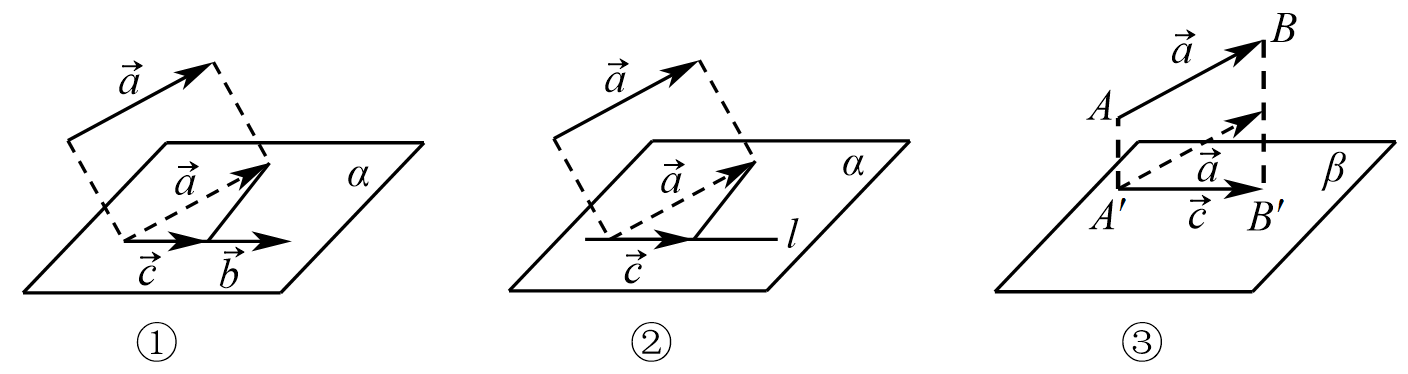
\includegraphics[width=84.0mm]{figs/sub3_B_4.png}}\par\vspace{-1.0mm}\penalty10000

\bindp (3)向量\(\overrightarrow{a}\)向平面\(\beta\)投影：

\bindp 如图③，分别由向量\(\overrightarrow{a}\)的起点\emph{A}和终点\emph{B}作平面\(\beta\)的垂线，垂足分别为\(A'\)，\(B'\)，得到向量\(\overrightarrow{A'B'}\)，向量\(\overrightarrow{A'B'}\)称为向量\(\overrightarrow{a}\)在平面\(\beta\)上的投影向量.\par\addvspace{0.80mm}

\begin{ansblock}[导-课时02-预习填空]
% ans:导-课时02-预习填空
\ansnote{预习填空}{知识点一：\(0^{\circ}\le\langle\overrightarrow{a},\overrightarrow{b}\rangle\le180^{\circ}\)；垂直。知识点二：零向量；\(\overrightarrow{b}\cdot\overrightarrow{a}\)；\(\lambda\)；\(\overrightarrow{a}\cdot\overrightarrow{c}+\overrightarrow{b}\cdot\overrightarrow{c}\)。知识点三：无空。}
\end{ansblock}

\zhenhead{判断正误(正确的打\gou{},错误的打\cha{})}

\zhentib{(1)}{向量\(\overrightarrow{a}\)在向量\(\overrightarrow{b}\)上的投影向量是与\(\overrightarrow{a}\)共线的向量．}

\zhentib{(2)}{若\(\overrightarrow{a}\perp\overrightarrow{b}\)，则向量\(\overrightarrow{a}\)在向量\(\overrightarrow{b}\)上的投影向量为\(\overrightarrow{0}\)．}

\begin{ansblock}[导-课时02-判5]
% ans:导-课时02-判5
\ansitem{(5)}{$\times$}
\anssub{(6)}{\(\surd\)}
\end{ansblock}

\liubai[9mm]{此处书写}

% ---------- 课中探究（探究点 5 个：例1→变式1→素养小结；题面逐字承 v11 冻结件探究点五~九） ----------
\huaxing{课}{中}{探}{究}{考点探究\quad 素养小结}

\tjdnr{一}{数量积的概念与运算律}{例\textbf{1}\duoxuan}{简单(知识点二)}{设\(\overrightarrow{a}\)，\(\overrightarrow{b}\)为空间中的任意两个非零向量，下列各式中正确的有(\kongwei)}

\bindopt {\fontsize{10.5pt}{19pt}\selectfont A．\({\overrightarrow{a}}^{2} = | \overrightarrow{a} |^{2}\)；\par}

\bindopt {\fontsize{10.5pt}{19pt}\selectfont B．\(\frac{\overrightarrow{a} \cdot \overrightarrow{b}}{\overrightarrow{a} \cdot \overrightarrow{a}} = \frac{\overrightarrow{b}}{\overrightarrow{a}}\)；\par}

\bindopt {\fontsize{10.5pt}{19pt}\selectfont C．\(( \overrightarrow{a} \cdot \overrightarrow{b} )^{2} = {\overrightarrow{a}}^{2} \cdot {\overrightarrow{b}}^{2}\)；\par}

\bindopt {\fontsize{10.5pt}{19pt}\selectfont D．\(( \overrightarrow{a} - \overrightarrow{b} )^{2} = {\overrightarrow{a}}^{2} - 2\overrightarrow{a} \cdot \overrightarrow{b} + {\overrightarrow{b}}^{2}\)\par}

\liubai[6mm]{解答书写区}

\begin{ansblock}[导-课时02-探1-例1]
% ans:导-课时02-探1-例1
\ansnote{例1}{AD}
\end{ansblock}

\liB{变式\textbf{1}}{简单(知识点二)}{}{已知\(|\overrightarrow{a}|=2\)，\(|\overrightarrow{b}|=3\)，\(\langle\overrightarrow{a},\overrightarrow{b}\rangle=60^\circ\)，则\nobreak\((\overrightarrow{a}+2\overrightarrow{b})\cdot(\overrightarrow{a}-\overrightarrow{b})=\)\kongbai{}.}

\begin{ansblock}[导-课时02-探1-变式1]
% ans:导-课时02-探1-变式1
\ansnote{变式1}{\(-11\)}
\end{ansblock}

\xiaojie{①识别：题干列出数量积相关的若干等式(平方、商式、乘积展开)要求判断正误时，判归本题型.}

\bindpx {\kaishu ②操作：按定义a·b=|a||b|cosθ逐式展开核验，展开后移项验算.}

\bindpx {\kaishu ③收束：警惕向量无除法、数量积无结合律等误用.}

\tjdnr{二}{数量积求夹角与投影}{例\textbf{1}}{中档(知识点一)}{如图，在正方体\(ABCD\text{-}\penalty100 A_{1}B_{1}C_{1}D_{1}\)中，求向量\(\overrightarrow{BC_{1}}\)与\(\overrightarrow{AC}\)的夹角的大小.}

\bindp \par\vspace{1.9mm}\penalty10000\noindent\makebox[\linewidth][c]{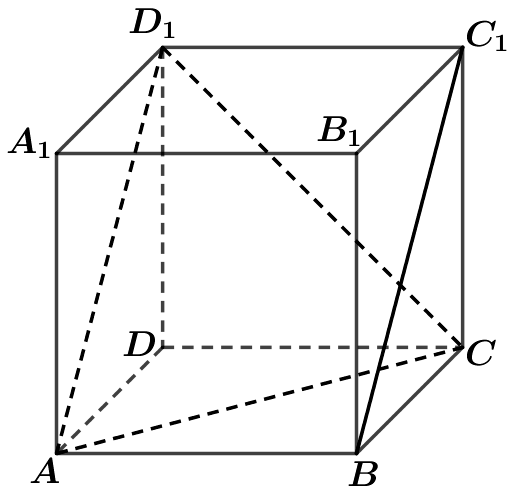
\includegraphics[width=54.1mm]{figs/image3.png}}\par\vspace{-1.0mm}\penalty10000

\liubai[6mm]{解答书写区}

\begin{ansblock}[导-课时02-探2-例1]
% ans:导-课时02-探2-例1
\ansnote{例1}{\(60^{\circ}\)}
\end{ansblock}

\liB{变式\textbf{1}}{中档(知识点一)}{}{在长方体\(ABCD\text{-}\penalty100 A_1B_1C_1D_1\)中，\(AB=2\)，\(AD=2\)，\(AA_1=1\)，则向量\(\overrightarrow{AB_1}\)与\(\overrightarrow{AC}\)夹角的余弦值为\kongbai{}.}

\begin{ansblock}[导-课时02-探2-变式1]
% ans:导-课时02-探2-变式1
\ansnote{变式1}{\(\dfrac{\sqrt{10}}{5}\)}
\end{ansblock}

\xiaojie{①识别：题干在几何体中求两向量的夹角、模长或投影而不建坐标系时，判归本题型.}

\bindpx {\kaishu ②操作：先平移向量使起点共点或选不共面的三个向量作基底，再把相关向量用基底表示并算出数量积与模长.}

\bindpx {\kaishu ③收束：最后代入夹角公式并按向量夹角范围[0,π]取角.}

\tjdnr{三}{数量积条件求参}{例\textbf{1}}{中档(知识点二)}{已知向量\(\overrightarrow{a},\overrightarrow{b}\)，且\(| \overrightarrow{a} | = 2\)，\(| \overrightarrow{b} | = 1\)，\(\langle \overrightarrow{a},\overrightarrow{b} \rangle = 60^{\circ}\)，则使向量\(\overrightarrow{a} + \lambda\overrightarrow{b}\)与\(\lambda\overrightarrow{a} - 2\overrightarrow{b}\)的夹角为钝角的实数\(\lambda\)的取值范围是\kongbai{}.}

\liubai[6mm]{解答书写区}

\begin{ansblock}[导-课时02-探3-例1]
% ans:导-课时02-探3-例1
\ansnote{例1}{\((-1-\sqrt{3},\,-1+\sqrt{3})\)}
\end{ansblock}

\liB{变式\textbf{1}}{简单(知识点二)}{}{已知\(| \overrightarrow{a} | = 3\sqrt{2},| \overrightarrow{b} | = 4,\overrightarrow{m} = \overrightarrow{a} + \overrightarrow{b},\overrightarrow{n} = \overrightarrow{a} + \lambda\overrightarrow{b},\langle \overrightarrow{a},\overrightarrow{b} \rangle = 135{^\circ},\overrightarrow{m}\bot\overrightarrow{n}\)，则λ=\kongbai{}.}

\begin{ansblock}[导-课时02-探3-变式1]
% ans:导-课时02-探3-变式1
\ansnote{变式1}{\(-\dfrac{3}{2}\)}
\end{ansblock}

\xiaojie{①识别：题干给出两向量的模与夹角、并以夹角为锐角/钝角或两向量垂直为条件求参数时，判归本题型.}

\bindpx {\kaishu ②操作：第一步用数量积把条件翻译成不等式或方程(锐角cos>0、钝角cos<0、垂直cos=0).}

\bindpx {\kaishu ③收束：再求解并剔除使两向量共线的参数，最后写出参数值或取值范围.}

\tjdnr{四}{数量积求距离(展开法)}{例\textbf{1}}{中档(知识点二)}{如图，在大小为45°的二面角A\-EF\-D中，四边形ABFE，CDEF都是边长为1的正方形，则B，D两点间的距离是\nobreak(\kongwei)}

\bindp \par\vspace{1.9mm}\penalty10000\noindent\makebox[\linewidth][c]{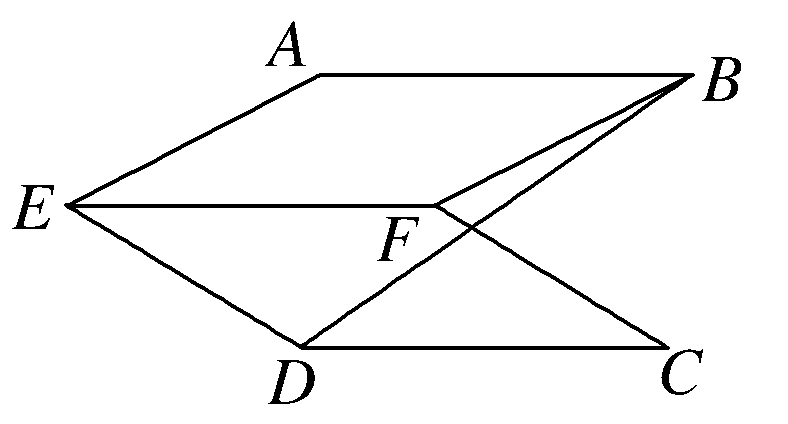
\includegraphics[width=47.5mm]{figs/image4.png}}\par\vspace{-1.0mm}\penalty10000

\bindopt {\fontsize{10.5pt}{19pt}\selectfont \makebox[\dimexpr0.5\linewidth-1em\relax][l]{A．\(\sqrt{3}\)；}\makebox[\dimexpr0.5\linewidth-1em\relax][l]{B．\(\sqrt{2}\)；}\par}

\bindopt {\fontsize{10.5pt}{19pt}\selectfont \makebox[\dimexpr0.5\linewidth-1em\relax][l]{C．1；}\makebox[\dimexpr0.5\linewidth-1em\relax][l]{D．\(\sqrt{3 - \sqrt{2}}\)}\par}

\liubai[6mm]{解答书写区}

\begin{ansblock}[导-课时02-探4-例1]
% ans:导-课时02-探4-例1
\ansnote{例1}{D}
\end{ansblock}

\liB{变式\textbf{1}}{简单(知识点二)}{}{在大小为\(60^\circ\)的二面角\(A\text{-}\penalty100 EF\text{-}\penalty100 D\)中，四边形\(ABFE\)，\(CDEF\)都是边长为\(1\)的正方形，则\nobreak\(B\)，\(D\)两点间的距离为\kongbai{}.}

\begin{ansblock}[导-课时02-探4-变式1]
% ans:导-课时02-探4-变式1
\ansnote{变式1}{\(\sqrt{2}\)}
\end{ansblock}

\xiaojie{①识别：题干在含二面角的拼接图形中求两点距离时，判归本题型.}

\bindpx {\kaishu ②操作：第一步把待求线段对应的向量写成已知棱向量的首尾相接和链，再对模长平方作数量积展开，逐项代入模长与夹角(端点处两条垂线段的夹角由二面角决定，注意取45°还是135°).}

\bindpx {\kaishu ③收束：最后开方得距离.}

\tjdnr{五}{数量积求距离(折叠矩形)}{例\textbf{1}}{中档(知识点二)}{已知矩形\(ABCD\)中，\(AB = 1\)，\(BC = \sqrt{3}\)，将矩形\(ABCD\)沿对角线\(AC\)折起，使平面\(ABC\)与平面\(ACD\)垂直，则\nobreak\(|\overrightarrow{BD}| =\)(\kongwei).}

\bindopt {\fontsize{10.5pt}{19pt}\selectfont \makebox[\dimexpr0.25\linewidth-0.5em\relax][l]{A．\(\frac{\sqrt{10}}{2}\)；}\makebox[\dimexpr0.25\linewidth-0.5em\relax][l]{B．\(\frac{\sqrt{6}}{2}\)；}\makebox[\dimexpr0.25\linewidth-0.5em\relax][l]{C．\(\frac{\sqrt{5}}{2}\)；}\makebox[\dimexpr0.25\linewidth-0.5em\relax][l]{D．2}\par}

\liubai[6mm]{解答书写区}

\begin{ansblock}[导-课时02-探5-例1]
% ans:导-课时02-探5-例1
\ansnote{例1}{A}
\end{ansblock}

\liB{变式\textbf{1}}{中档(知识点二)}{}{已知矩形\(ABCD\)中，\(AB=1\)，\(BC=\sqrt{3}\)，将矩形\(ABCD\)沿对角线\(AC\)折起，使二面角\(B\text{-}\penalty100 AC\text{-}\penalty100 D\)的大小为\(60^\circ\)，则\nobreak\(|\overrightarrow{BD}|=\)\kongbai{}.}

\begin{ansblock}[导-课时02-探5-变式1]
% ans:导-课时02-探5-变式1
\ansnote{变式1}{\(\dfrac{\sqrt{7}}{2}\)}
\end{ansblock}

\xiaojie{①识别：题干为平面图形沿一条直线折起且折后两面垂直、求两点间距离时，判归本题型.}

\bindpx {\kaishu ②操作：第一步在折后图形中过两点对折痕作垂线定出垂足，再把目标向量写成两段垂线与折痕段的和链并平方展开.}

\bindpx {\kaishu ③收束：最后利用面面垂直带来的向量垂直逐项化简、开方得距离.}

% ---------- 课堂评价（恒 5 题＝3 单选＋2 填空；难度≤例题；提示词形制；本轮命制·逐题亲算——见 S2就绪报告 附录A） ----------
\begin{ketang}{本组共5题，1—3为单选，4—5为填空．}

\jiancestem{{\fontsize{11.4pt}{14pt}\selectfont\heihao {\numboldjian 1}．}\hspace{4.1mm}\tieside{简单(知识点二)}\hspace{2.2mm}已知\(|\overrightarrow{a}|=2\)，\(|\overrightarrow{b}|=1\)，且\(\overrightarrow{a}+\overrightarrow{b}\)与\(\overrightarrow{b}\)垂直，则\nobreak\(\overrightarrow{a}\cdot\overrightarrow{b}=\)(\kongwei)}

\bindopt {\fontsize{10.5pt}{21pt}\selectfont \makebox[\dimexpr0.25\linewidth-0.5em\relax][l]{A．\(-1\)；}\makebox[\dimexpr0.25\linewidth-0.5em\relax][l]{B．\(1\)；}\makebox[\dimexpr0.25\linewidth-0.5em\relax][l]{C．\(-2\)；}\makebox[\dimexpr0.25\linewidth-0.5em\relax][l]{D．\(2\)}\par}

\begin{ansblock}[导-课时02-评1]
% ans:导-课时02-评1
\ansitem{1}{A（\(-1\)）}
\end{ansblock}

\jiancestem{{\fontsize{11.4pt}{14pt}\selectfont\heihao {\numboldjian 2}．}\hspace{4.1mm}\tieside{简单(知识点二)}\hspace{2.2mm}设\(\overrightarrow{a}\)，\(\overrightarrow{b}\)均为非零空间向量，则“\(\overrightarrow{a}\cdot\overrightarrow{b}=0\)”是“\(|\overrightarrow{a}+\overrightarrow{b}|=|\overrightarrow{a}-\overrightarrow{b}|\)”的(\kongwei)}

\bindopt {\fontsize{10.5pt}{21pt}\selectfont \makebox[\dimexpr0.5\linewidth-1em\relax][l]{A．充分不必要条件；}\makebox[\dimexpr0.5\linewidth-1em\relax][l]{B．必要不充分条件；}\par}

\bindopt {\fontsize{10.5pt}{21pt}\selectfont \makebox[\dimexpr0.5\linewidth-1em\relax][l]{C．充要条件；}\makebox[\dimexpr0.5\linewidth-0.5em\relax][l]{D．既不充分也不必要条件}\par}

\begin{ansblock}[导-课时02-评2]
% ans:导-课时02-评2
\ansitem{2}{C（充要）}
\end{ansblock}

\jiancestem{{\fontsize{11.4pt}{14pt}\selectfont\heihao {\numboldjian 3}．}\hspace{4.1mm}\tieside{简单(知识点一)}\hspace{2.2mm}已知非零空间向量\(\overrightarrow{a},\overrightarrow{b}\)满足\(|\overrightarrow{a}|=|\overrightarrow{b}|=2\)，\(\overrightarrow{a}\cdot\overrightarrow{b}=2\)，则\nobreak\(\langle\overrightarrow{a},\overrightarrow{b}\rangle=\)(\kongwei)}

\bindopt {\fontsize{10.5pt}{21pt}\selectfont \makebox[\dimexpr0.25\linewidth-0.5em\relax][l]{A．\(30^\circ\)；}\makebox[\dimexpr0.25\linewidth-0.5em\relax][l]{B．\(45^\circ\)；}\makebox[\dimexpr0.25\linewidth-0.5em\relax][l]{C．\(60^\circ\)；}\makebox[\dimexpr0.25\linewidth-0.5em\relax][l]{D．\(90^\circ\)}\par}

\begin{ansblock}[导-课时02-评3]
% ans:导-课时02-评3
\ansitem{3}{C（\(60^{\circ}\)）}
\end{ansblock}

\jiancestem{{\fontsize{11.4pt}{14pt}\selectfont\heihao {\numboldjian 4}．}\hspace{4.1mm}\tieside{简单(知识点三)}\hspace{2.2mm}已知\(|\overrightarrow{a}|=4\)，\(\overrightarrow{a}\)与\(\overrightarrow{b}\)的夹角为\(60^\circ\)，则向量\(\overrightarrow{a}\)在向量\(\overrightarrow{b}\)上的投影向量的模为\kongbai{}．{\zhushi{(提示：投影向量与\(\overrightarrow{b}\)共线，其模为\(|\overrightarrow{a}|\,|\cos\langle\overrightarrow{a},\overrightarrow{b}\rangle|\))}}}

\begin{ansblock}[导-课时02-评4]
% ans:导-课时02-评4
\ansitem{4}{2}
\end{ansblock}

\jiancestem{{\fontsize{11.4pt}{14pt}\selectfont\heihao {\numboldjian 5}．}\hspace{4.1mm}\tieside{中档(知识点二)}\hspace{2.2mm}已知\(|\overrightarrow{a}|=2\)，\(|\overrightarrow{b}|=1\)，\(\langle\overrightarrow{a},\overrightarrow{b}\rangle=120^\circ\)，则\nobreak\((2\overrightarrow{a}-\overrightarrow{b})\cdot(\overrightarrow{a}+3\overrightarrow{b})=\)\kongbai{}．{\zhushi{(提示：按运算律展开，其中\(\overrightarrow{a}\cdot\overrightarrow{b}=|\overrightarrow{a}||\overrightarrow{b}|\cos\langle\overrightarrow{a},\overrightarrow{b}\rangle\))}}}

\begin{ansblock}[导-课时02-评5]
% ans:导-课时02-评5
\ansitem{5}{0}
\end{ansblock}

\end{ketang}

\end{multicols}

\tailfill
\end{document}
